% File project.tex
%% Style files for ACL 2021
\documentclass[11pt,a4paper]{article}
\usepackage[hyperref]{acl2021}
\usepackage{times}
\usepackage{booktabs}
\usepackage{todonotes}
\usepackage{latexsym}
\renewcommand{\UrlFont}{\ttfamily\small}

% Added by Yanlin
\usepackage{amsmath,amssymb}
\usepackage{graphicx}
\usepackage{caption}
\usepackage{subcaption}
\usepackage{threeparttable}

% This is not strictly necessary, and may be commented out,
% but it will improve the layout of the manuscript,
% and will typically save some space.
\usepackage{microtype}

\aclfinalcopy 

\newcommand\BibTeX{B\textsc{ib}\TeX}

\title{11-777 Report 2: Related Work and Model Proposal}

\author{
  Hao Wu\thanks{\hspace{4pt}Everyone Contributed Equally -- Alphabetical order} \hspace{2em} Jiayi Shen$^*$ \hspace{2em} Yanlin Feng$^*$ \hspace{2em} Yinghuan Zhang$^*$ \hspace{2em} Yuwei Wu$^*$\\
  \texttt{\{haowu3, jiayis2, yanlinf, yinghuan, yuweiwu\}@andrew.cmu.edu}
  }

\date{}

\begin{document}
\maketitle
\section{Related Work and Background}
\subsection{Related Datasets}

\paragraph{TextVQA, TextVQA-X, and TextCaps} TextVQA\footnote{See https://textvqa.org/ for details.} contains 28,408 images from OpenImages and 45,336 questions that require reading and reasoning about text in images. Each question comes with 10 ground truth answers. TextVQA-X \cite{rao2021first} contains 11,681 images and 15,374 questions from TextVQA. For each question, up to 5 distinct human annotators provide visual and textual explanations for why a given answer is correct. TextCaps \cite{sidorov2020textcaps} is another dataset that is built upon TextVQA. 5 captions are collected for each image in the TextVQA dataset.

\paragraph{ST-VQA} Created with a similar purpose as that of TextVQA, ST-VQA \cite{biten2019scene} comprises 23,038 images sourced from six datasets and 31,791 questions that can be unambiguously answered using text in the image. (In contrast, 39\% of the answers in TextVQA do not contain OCR tokens.) Each question comes with up to 2 ground truth answers. 

\paragraph{VQA v2.0} As an updated version of the first large-scale VQA dataset, VQA v2.0\footnote{See https://visualqa.org/ for details.} contains 265,016 images and abstract scenes, 204,721 of which are COCO images. While there are a total of 1,105,904 questions, only 8k (or less than 1\%) of these questions require reading text in the image \cite{biten2019scene}. Each question comes with 10 ground truth answers.

\paragraph{OCR-CC} Another large-scale dataset worth mentioning is the OCR-CC dataset \cite{yang2021tap}. It contains 1.367 million scene text-related image-caption pairs from the Conceptual Captions dataset. The scene text detected per image has a mean and median of 11.4 and 6, compared with 23.1 and 12 in TextVQA, and 8.03 and 6 in ST-VQA.

\paragraph{VisualMRC} Recently \citet{tanaka2021visualmrc} proposed the VisualMRC dataset which is a machine reading comprehension dataset based on document images. VisualMRC contains long abstractive answers which do not correspond to spans in the documents. Images in VisualMRC are sourced from multiple domains which makes it more challenging than DocVQA.


\subsection{Unimodal Baselines}
\paragraph{Question} When only using the question module and predicting from the 8000 most frequent answers, LoRRA \cite{Singh_2019_CVPR} achieves validation and test accuracies of 8.09\% and 8.70\%. 

\paragraph{Image} When only using the image module and predicting from the 8000 most frequent answers, LoRRA achieves validation and test accuracies of 6.29\% and 5.58\%. 

\paragraph{OCR} LoRRA uses Rosetta-ml to produce OCR tokens. By predicting a random OCR token present in an image, validation and test accuracies of 7.72\% and 9.12\% are achieved. By predicting the most frequently occurring OCR token in an image, validation and test accuracies of 9.76\% and 11.60\% are achieved.


\subsection{Relevant techniques}
\subsubsection{Feature extraction}
\paragraph{Question Embedding} Pretrained language models \cite{devlin2018bert} have become the dominant text encoders in recent work. These models are trained on massive amount of unlabeled text by minimizing unidirectional or bidirectional language modeling loss and later finetuned on specific domains.
\paragraph{Regional Image Feature}
Faster R-CNN model is the dominant approach used in VQA related tasks to extract region-based object features, including visual information (convolutional features), positional information (bounding box coordinates) and class labels of detected objects. 
Apart from feature information on detected objects, there are papers such as \citet{gao2020multi} that extract grid-based features as visual embedding, which mainly relies on ResNet and its variants to learn image representation as 2048-D vectors corresponding to 196 grids.

\paragraph{Whole Image Feature}\citet{rao2021first} uses Feature Pyramid Network (FPN) to construct a semantic segmentation of the image and obtain visual explanations.
In addition, although not mentioned in the VQA papers covered in this literature review, depth map is another potentially meaningful representation of the whole image besides RGB information, towards which Dense Prediction Transformer (DPT) (\citet{DenseViT}) is the state-of-the-art approach to estimate fine-grained depth information based on an architecture combining vision transformer encoder and convolutional decoder. 

\paragraph{OCR System}OCR methods used in prior work include Rosetta-en OCR, Rosetta-ml OCR, SBD-Trans OCR, and Google-OCR. While LoRRA \cite{Singh_2019_CVPR} only uses FastText to extract word embedding from the OCR tokens, M4C and many later models employ a multi-feature representation, including appearance feature extracted using Faster R-CNN, character feature extracted using Pyramidal Histogram of Characters (PHOC), and a 4-dimensional location feature of the token’s relative bounding box coordinates. In addition, \citet{gao2021sma} introduced a 512D CNN feature called RecogCNN, which is extracted from text visual patches and trained on a text recognition task. 

\subsubsection{Multimodal Multitask Learning}
There has been progresses made in the area of multimodal multi-task learning. \citet{lu202012} jointly trained 12 vision-and-language tasks with a multi-task transformer based on VILBERT \cite{lu2019vilbert}. \citet{hu2021unit} further expanded beyond fixed input modalities and jointly handled different single modal and multimodal tasks with a unified transformer model. They also pointed out the multimodal tasks such as VQA benefit from multi-task traning with uni-modal tasks.

Besides jointly training on tasks from different domains, several works designed a variety of highly correlated tasks to enhance the performance of VQA models.

\paragraph{Bounding Box Prediction}\citet{han2020finding} introduces a bounding box prediction task to prove its confidence of answer prediction. Specifically, when the model generates the answer by copying from OCR tokens, the IoU between the predicted bounding box and the ground truth OCR bounding box is calculated, serving as an evidence. The loss the IoU is added into training loss to urge the model to predict credible answer.

\paragraph{ANLS As Reward}Average Normalized Levenshtein Similarity (ANLS) is another popular metric in TextVQA task. It is used to measure the similarity between predicted answer and ground truth answer instead of binary comparison. It is common case that OCR system provides an incorrect token that model fail to get the exact correct answer due to the systematic error. ANLS guides the model to make the right prediction even when the predicted answer does not exactly match it ground truth. Many prior works\cite{zhu2020simple, liu2020cascade} introduced ANLS as a reward into the training loss.

\subsubsection{Attention mechanisms}
Graph Attention Networks (GAT)\cite{velivckovic2017graph} is broadly used in prior works to encode visual relationship between objects, which has proven to be crucial to many computer vision tasks. ReGAT\cite{li2019regat} introduces a Relation-aware GAT to model multi-type inter-object relations, including positional relation, semantic interactions and implicit relations. SA-M4C\cite{kant2020spatially} improves M4C by introducing spatially aware self-attention layer where objects attend each other in a spatial graph.

Visual relation is important, though, TextVQA task requires a better understanding of relationship across multiple modalities. Many previous works explored relations between objects and OCR under the question text supervision. CRN\cite{liu2020cascade} feeds question text features, OCR text features, and visual features into the Progressive Attention Module in turn and update informative features gradually. SSBaseline\cite{zhu2020simple} encodes multimodal features with three attention blocks, in each block OCR visual features, OCR text features, and object features attended with question embedding respectively. SMA\cite{gao2021sma} uses a Question Conditioned Graph Attention Module to encoder the object-object, object-OCR, OCR-OCR relationships under the question's guidance. 

\subsubsection{Pre-training}
Given that our target task requires reasoning over both text and images, our main focus here is the Vision-and-Language Pre-training (VLP). There are several strategies commonly used to train VLP models.

\paragraph{Image Text Matching} This task requires the model to generate high-quality instance-level representations. Given a random pair of image and text descriptions, the model predicts whether the pair is matched. This task is widely used in a vartity of VLP models including ViLT, TAP, VISUALBERT, VILBERT, and LXMERT \cite{kim2021vilt, yang2021tap, li2019visualbert, lu2019vilbert, tan2019lxmert}. LayoutLM \cite{xu2020layoutlm} further modified this task into Multi-label document classification task and used the document tags to supervise the document-level representation learning. 

\paragraph{Masked Language Modeling} Following the mechanisms proposed by \citet{kenton2019bert}, this objective aims at predicting masked text tokens from the given contextualized vector and vectors corresponding to image regions. \citet{kim2021vilt} introduced whole word masking for MLM task to train VLP models, while \citet{powalski2021going} proposed to use T5-like salient span masking schema. \citet{lu2019vilbert, tan2019lxmert} extended this idea to masked multi-modal modeling task. In this manner, 15\% of both words and image region inputs are masked and the model is required to reconstruct given the remaining inputs. 

\paragraph{Other Cross-Modality Tasks}  Addition to the above prediction tasks, a few models also introduce several tasks that need strong cross-modality representations. \citet{xu2021layoutlmv2} proposed a text-image alignment task to encourage the model learn the alignment of detected objects among different modalities. \citet{yang2021tap} designed a relative (spatial) position prediction (RPP) task. The RPP task aims to predict the relative spatial position between an object region and a scene text region. \citet{tan2019lxmert} proposed image question answering tasks on the pretraining stage to further enhance the cross-modality representations.


% TAP performed three scene text-aware pre-training tasks. For scene-text language pre-training, the authors designed a masked language modeling (MLM) task and an image-text (contrastive) matching (ITM) task. The extended text input includes question text, detected object labels, and detected scene text words. Specifically, the MLM task aims to recover the masked words. The ITM task aims to predict if a text sequence has been partially replaced. 
% For scene-text visual pre-training, they designed a relative (spatial) position prediction (RPP) task. The RPP task aims to predict the relative spatial position between an object region and a scene text region.

\subsubsection{Multireference}
\citet{rao2021first} uses the sample one technique to leverage the multiple textual explanations collected for each question. In each training epoch, one of the available textual explanations is randomly selected.

\subsubsection{Copy Mechanism and Pointer Network}

Many sequence learning tasks requires \textit{copying}, which refers to selectively replicating segments of the input to generate the output. For example, in a dialogue system, the agent needs to generate responds by referring to entities in the input utterance. Another example is text summarization, where the model is required to extract text from the original documents. Similar phenomenon is also observed in real-world language communication where humans tend to repeat long phrases in conversation.

Various pointer network \cite{vinyals2015pointer} architectures have been proposed to address the challenge of \textit{copying}. \citet{gu2016incorporating} proposed {CopyNet} to address copying in seq2seq learning tasks. {CopyNet} generates an answer token at each timestep based on a mix of generation-mode probabilities and copy-mode probabilities, where the copy-mode probabilities are computed by attending to the input tokens. \citet{see2017get} generalized CopyNet by modeling the selection between generation and copyping with a binary classifier. 

Copying is also critical in text-related VQA tasks, where the answers often include OCR tokens in the image. LORRA \cite{Singh_2019_CVPR} concatenates OCR tokens to the common word vocabulary and compute normalization over the new vocabulary. M4C \cite{hu2020iterative} also augments transformer with a dynamic pointer network which computes OCR token probabilities with a bilinear layer.


\subsubsection{Data Augmentation and Generalizability}
Apart from designing efficient and robust model structures, there are papers targeting the generalization capabilities of VQA models and proposing methods on data augmentation, evaluation and training procedure.

\paragraph{Data Augmentation}
For image augmentation, in addition to techniques commonly used in computer vision community (rotation, scaling, adding noises, etc), which typically don't affect the semantic meaning of the visual content, VQA image augmentation also involves transformations that deliver significantly different visual information. For instance, \citet{mutant} has proposed to mutate images via removing object instances or inverting colors, which is critical enough to lead to different answers to the questions. It is worth noting that removing object instances requires additional procedures using inpainting network based on Generative Adversarial Network (GAN) to make transformed images photorealisitic.  

As for questions augmentation, \citet{mutant} has adopted template-based questions operators to perform tasks such as negation on yes-no questions and substitution of critical words with antonyms. Moreover, \citet{RAD} followed another template-based approach that converts "what/how" questions into "yes/no" questions.  

\paragraph{Evaluation}
To measure and boost model performance on Out-Of-Distribution (OOD) datasets, several papers have come up with new metrics to evaluate generalizability. \citet{RAD} has introduced Robustness to Augmented Data (RAD), which calculates the proportion of correct answers on augmented samples among all correct answers, and has demonstrated the indicating power of RAD on model robustness against unseen data through quantitative results. 
Moreover, \citet{Roses} group questions on frequencies and argue that accuracy over infrequent question-answer pairs is more suitable in delineating generalization capabilites.   
 
\paragraph{Training Procedure}
The concept of grouping questions is not merely utilized in designing evaluation metrics, but adopted in the training procedure as well. For example,  \citet{mutant} has partitioned training samples by question types and optimized a different copy of the model under each cluster, which has been proved to lead to better out-of-distribution generalization. 

\section{Model Proposal}

\subsection{Overall model structure}
%%%%%%%%%%%%%%%%%%%%%%%%%%%%%%%%%%%%%%%%%%%%%%%%%%%%
\begin{figure*}[h]
  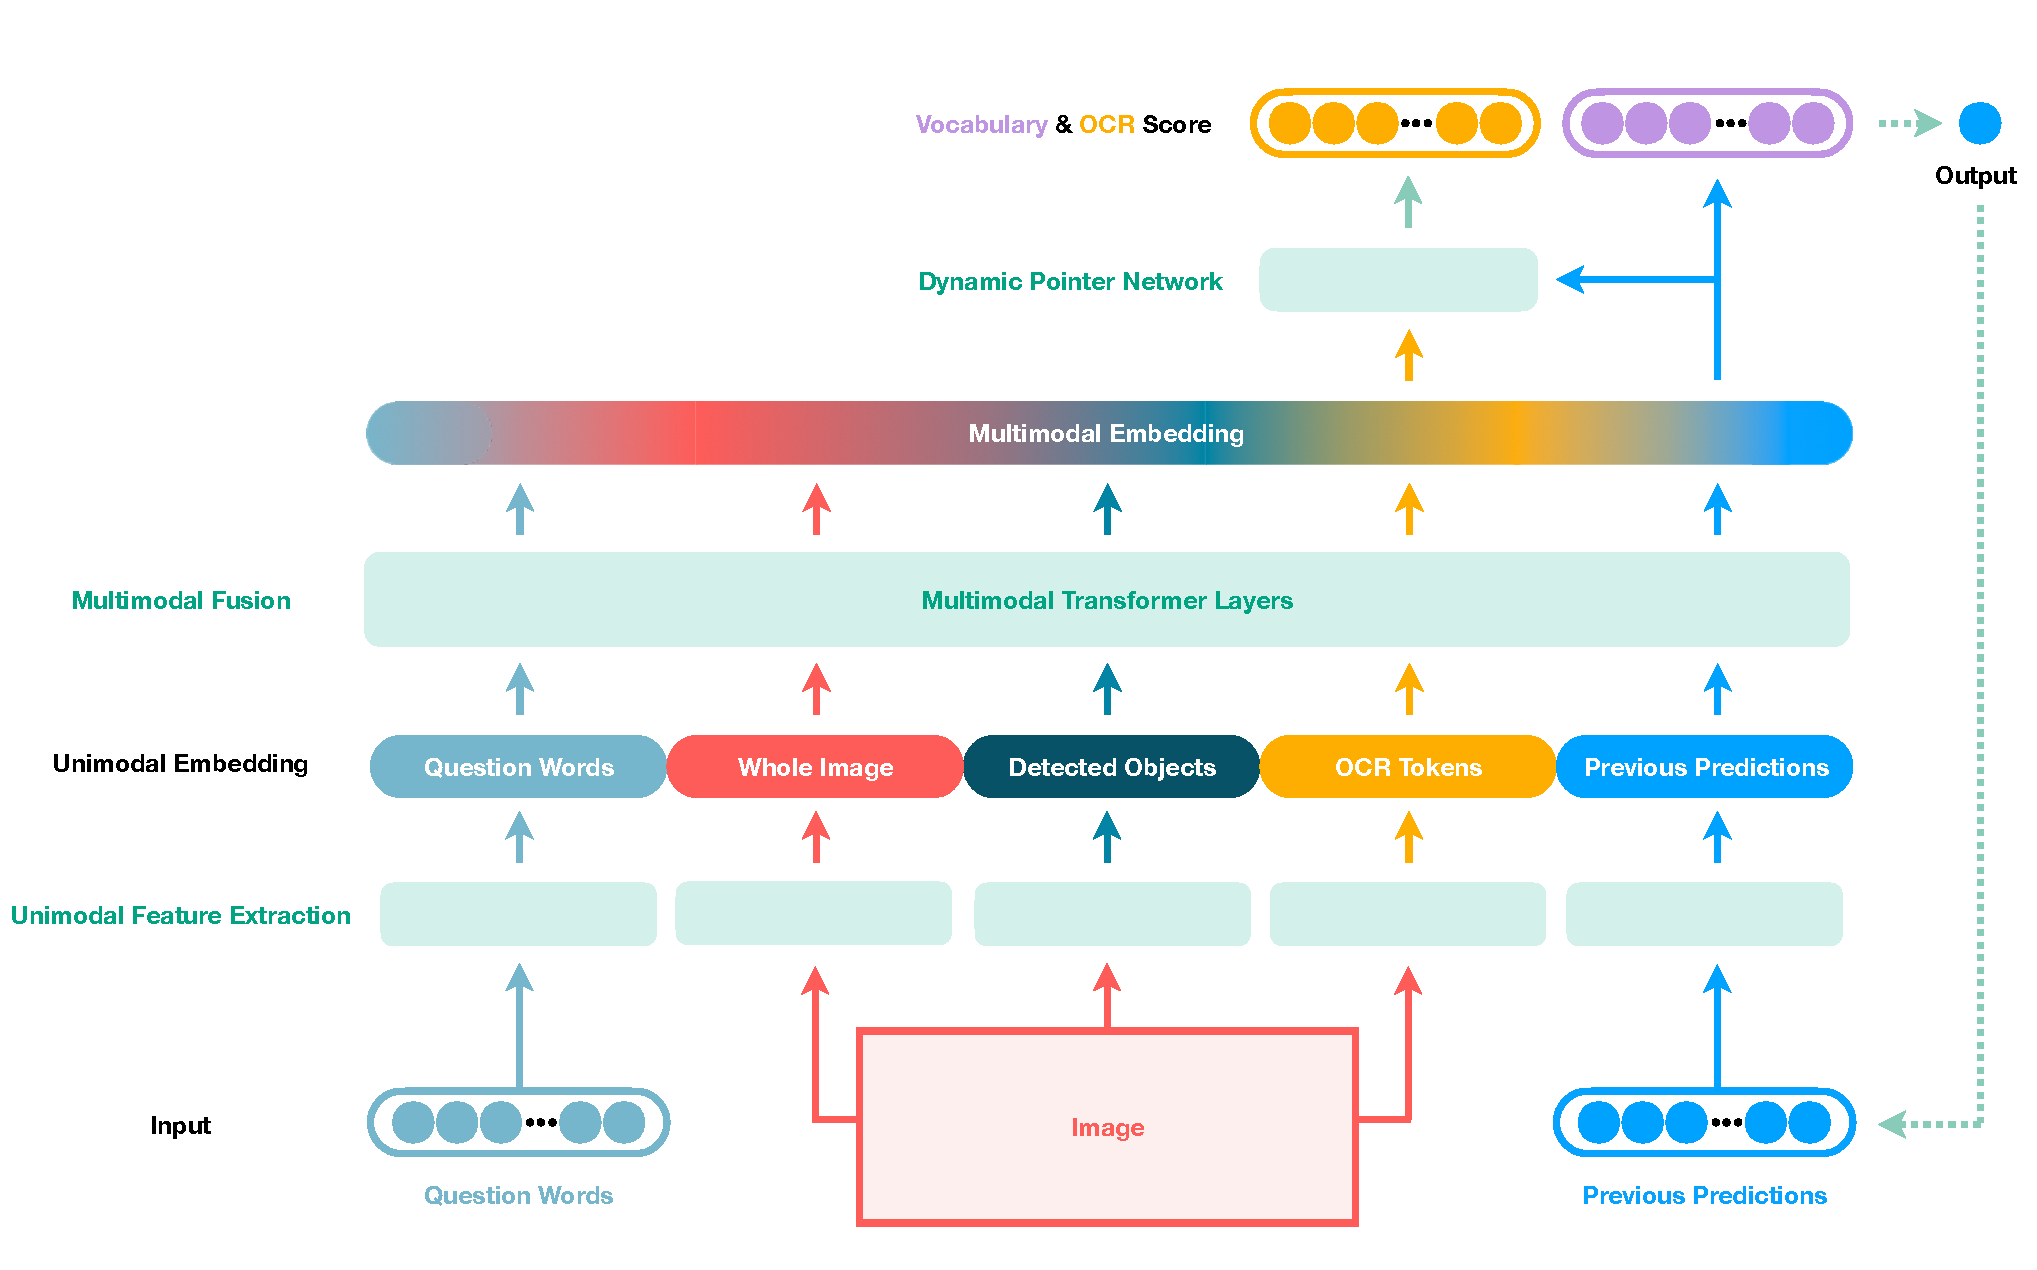
\includegraphics[width=\textwidth]{figures/ModelStructure.pdf}
  \caption{Overall Model Structure}
  \label{fig:model}
\end{figure*}
%%%%%%%%%%%%%%%%%%%%%%%%%%%%%%%%%%%%%%%%%%%%%%%%%%%%
We present our overall model structure as shown in Fig.\ref{fig:model}. Given a question and an image as input, we firstly extract the OCR tokens and object by an off-the-shelf OCR system and detector. We separately obtain the uni-modal features of all four modalities, including question, whole image, detected objects, and OCR tokens, and use one multimodal encoder to learn the multimodal embedding.

\subsection{Encoders}
Describe encoders for each modality and at least one alternatives for each.  Explain the relative strengths of each option (e.g. coverage, efficiency, ...)

\paragraph{Embedding of question words.}For question words, we follow the previous work and use the first $3$ layers of BERT-BASE, rather than all its $12$ layers, in order to save computation. Given a question with $W$ words, we embed it into a sequence of $d-$dimentional feature vector $\{x^{\textsuperscript{ques}}_i\}_{i=1}^W$. Alternatively, we can also use other pretrained language model of larger size like T5-Large model to get better question representations.

\paragraph{Embedding of whole image.} We introduce the entire image as a modality. We embed the entire image as a semantic segmentation map predicted by Feature Pyramid Network (FPN). Alternatively, the whole image can be represented as a depth map estimated by Dense Prediction Transformer (DPT), although semantic segmentation map may be able to encode more information and potentially advantageous in contributing to model performance. 

\paragraph{Embedding of detected objects.}Given an image, we obtain the region-based object features including visual features and bounding box features. These two parts features are extracted by an off-the-shelf Faster R-CNN. Visual features of $M$ objects are embedded into a sequence of same $d-$dimentional feature vector $\{x^{\textsuperscript{obj}}_{v,i}\}_{i=1}^M$ and another sequence of $4$-dimensional location feature vector $\{x^{\textsuperscript{obj}}_{bb,i}\}_{i=1}^M$ is used for bounding box location feature embedding. Alternatively, as implemented in \citet{gao2020multi}, a pretrained ResNet model can be used to extract grid-based image feature as a list of 196 $d-$dimentional vectors corresponding.    

In addition, we want to incorporate detected object labels. We use the same embedder as question texts to extract the label features of objects. A sequence of $d-$dimension feature vector $\{x^{\textsuperscript{obj}}_{label,i}\}_{i=1}^M$ is expected. 

\paragraph{Embedding of OCR tokens}For OCR tokens, we also plan to follow M4C and extract tokens using Rosetta-en. Specifically, we plan to use FastText for word embedding, Faster R-CNN for appearance feature, a 604-dimensional Pyramidal Histogram of Characters (PHOC) for character feature, and a 4-dimensional location feature of the token’s relative bounding box coordinates. Alternatively, we can use pretrained encoder like LayoutLM to encode the text, position and image features of OCR tokens. In this manner, the embedding of OCR tokens is jointly optimized compared with combining features from different modules like in M4C.

\paragraph{Multimodal Encoder} After obtaining embedding features of these four modalities, we use a typical encoder with $L-$layers stacked transformer layers as our multimodal encoder.

\subsection{Decoders}
We predict an answer with variable length based on M4C's dynamic network. Our multimodal encoder fuses features coming from four modalities, \textit{i.e.}, question words, whole image, detected objects, and OCR tokens, and outputs a multimodal feature vector as mentioned. In the decoding, we use exactly the same transformer layers as the multimodal encoder. A dynamic network takes this multimodal embedding as input to iteratively generate the answer. We construct a fixed vocabulary list of $V$ words which frequently appear in the training set answers and a dynamic case-ware vocabulary list of $N$ OCR tokens detected in the test image. The whole answer space at each inference is composed with these two vocabulary lists and additional two special tokens, \texttt{<begin>} and \texttt{<end>}.

At each time step, our decoder predicts one word from the case-aware answer space. The prediction begins with \texttt{<begin>} at time step $0$ which only takes multimodal embeddings as the input. For time step $t$, we feed the decoder both the multimodal embedding and the embedding of its previous prediction, and the next answer word coming from the case-aware answer space is generated based on the decoder output with a dynamic pointer network. We stop the decoding process after the decoder predict another special token \texttt{<end>}.

\subsection{Pretraining}  \label{subsec:pretrain}
According to \citet{yang2021tap}, pretraining on the same downstream task datasets, their system achieved an improvement of the absolute accuracy on the TextVQA dataset by +5.4\%. Inspired by this, we would like to implement several pretraining strategies over the TextVQA dataset to enhance our system's performance.

\paragraph{Masked Language Modeling} Inspired by \citet{kim2021vilt,powalski2021going}, we would like to use all input OCR tokens to perform the MLM tasks and in a salient whole word masking schema i.e. the whole words for named entities are preferred rather than random tokens . By masking these tokens, we encourage the system to predict meaningful entities from both the whole image and detected object features.

\paragraph{Masked Image Reconstruction} Similar to \citet{lu2019vilbert}, we would like to mask 15\% of the image region inputs and task the model with reconstructing the maksed image given the remaining inputs. The masked image regions are selected in the regions for detected objects and scene texts from the whole image.
%%%%%%%%%%%%%%%%%%%%%%%%%%%%%%%%%%%%%%%%%%%%%%%%%%%%
\begin{figure*}[h]
\centering
  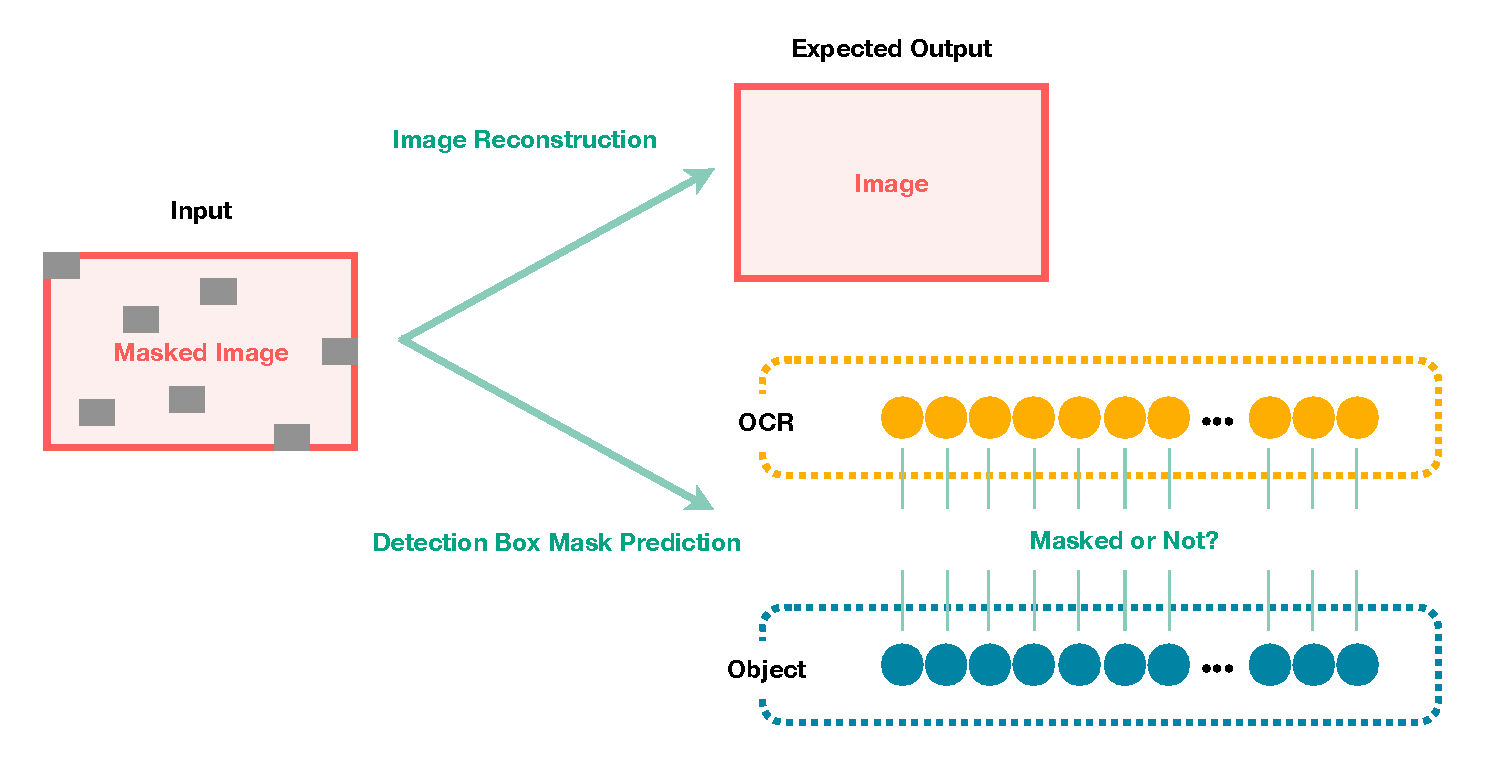
\includegraphics[width=0.8\textwidth]{figures/Pretraining_ImgRecon_DetectBoxMaskPred.pdf}
  \caption{Pretraining: Masked Image Reconstruction & Detection Box Mask Prediction.}
  \label{fig:pretraining_MIR}
\end{figure*}
%%%%%%%%%%%%%%%%%%%%%%%%%%%%%%%%%%%%%%%%%%%%%%%%%%%%

\paragraph{Image text matching} We would also like to implement the commonly used ITM task to help the model learn the correspondence between image and textual content. For ITM task, we would like to explore three different ways of constructing negative sample. The first one is to follow \citet{yang2021tap}'s way of polluting text words. The second way is to randomly replace detected objects while the last way is to randomly replace the whole image with ones from other training pairs.

\paragraph{Masked Box Position Prediction} In order to enhance the learning of relative positions among detected objects and OCR scene texts, we proposed a novel pretraining strategy called \textbf{masked box position prediction}. As shown in the figure \ref{fig:pretraining_PP}, we would randomly mask some of the position for detected objects and OCR scene texts. The system is required to predict the original coordinate for the masked positions. In this manner, we encourage the model to learn the relative position around the masked detection box.
%%%%%%%%%%%%%%%%%%%%%%%%%%%%%%%%%%%%%%%%%%%%%%%%%%%%
\begin{figure*}[h]
\centering
  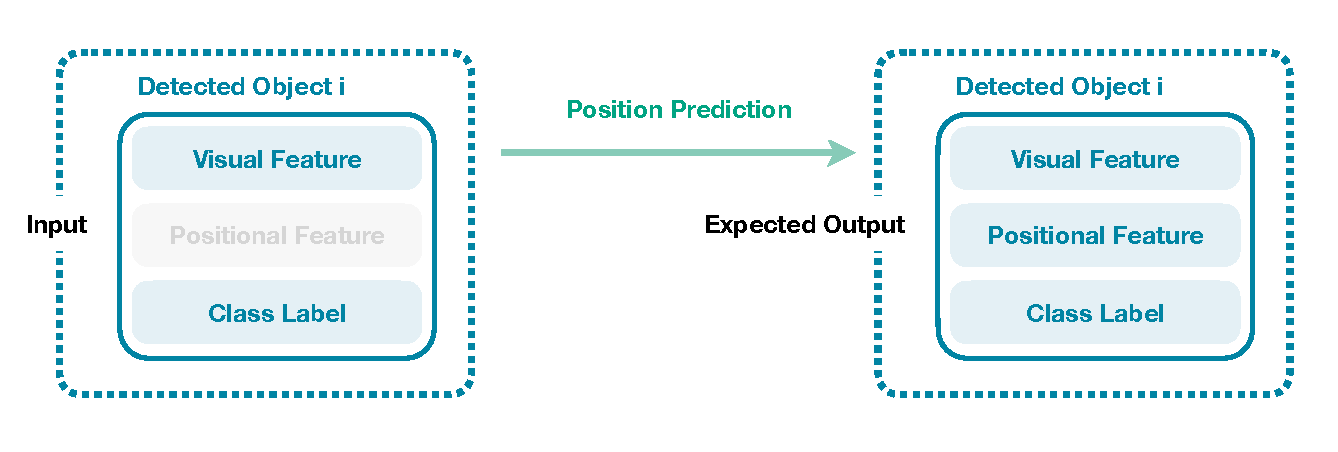
\includegraphics[width=0.7\textwidth]{figures/Pretraining_PositionPrediction.pdf}
  \caption{Pretraining: Position Prediction.}
  \label{fig:pretraining_PP}
\end{figure*}
%%%%%%%%%%%%%%%%%%%%%%%%%%%%%%%%%%%%%%%%%%%%%%%%%%%%

\paragraph{Image Text Alignment} This is another cross-modality pretraining task we would like to explore. In order to properly answer the questions in VQA dataset, it is essential to learn the alignment between OCR texts and whole image, the alignment between detected objects and whole image. So we proposed a new alignment task: \textbf{detection box mask prediction}. For detection box mask prediction, as illustrated in the figure \ref{fig:pretraining_MIR}, the image is processed in the same manner as in the masked image reconstruction task. The system is then required to predict whether each of the input OCR tokens and detected objects is masked in the whole image.


\subsection{Detecor/OCR-Robust Finetuning by Masking} \label{subsec:finetune}

While all TextVQA questions can be answer solely with the raw image, almost all models that have been proposed rely on pretrained object detectors and off-the-shelf OCR toolkits to provide information that is more fine-grain than the raw image. Such a strong dependency might hurt model performance if (1) the dataset domain differs significantly from the domain that the detector is trained on (2) the OCR recognizer produces poor results due to rotation or noises. Therefore, we propose to make our model more robust with respect to both the object detector and the OCR recognizer with a modality-specific masking strategy.

As illustrated in Figure \ref{fig:finetune}, the input image is represented in three different modalities: the raw image, objects  as well as OCR tokens. The objects (and the bounding box positions) are predicted by a pretrained detector like RCNN and the OCR tokens are extracted by an OCR recognizer. In textVQA, the question can \textit{always} be answered with only the raw image, while in most cases, can be answered with either of the other two modalities, given that the outputs from detector/OCR outputs are correct. \footnote{Note that some questions (e.g. clock reading questions) cannot be answered with only OCR even if the OCR results are correct.} Therefore, to avoid overfitting to objects or OCR tokens and thus make our model more robust w.r.t. to detector/OCR, we propose the following masking strategy during finetuning.

At each iteration, we randomly select one or two of the three modalities. For the selected modalities, we randomly mask $x$\% of the features by setting them to zeros. The model is required to predict the correct answer from the masked features. We finetune the model by minimizing the cross-entropy loss as in previous work. We believe this masking strategy will encourage model to utilize information in all three modalities thus reducing the risk of overfitting. Specifically, suppose the answer is one of the OCR tokens, masking it out will force the model to utilize information in the raw image to answer the question. As as result, our model will be more robust when the object detector or OCR recognizer behaves poorly.
%%%%%%%%%%%%%%%%%%%%%%%%%%%%%%%%%%%%%%%%%%%%%%%%%%%%
\begin{figure*}[h]
\centering
  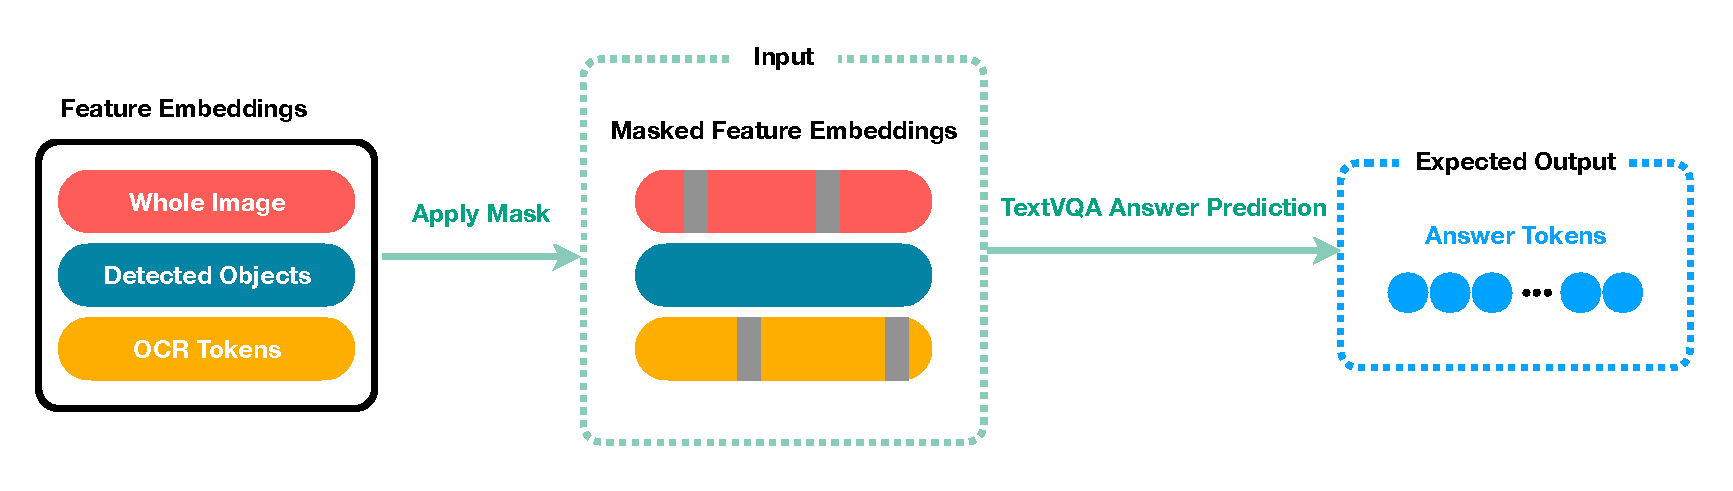
\includegraphics[width=0.8\textwidth]{figures/Multitask_FineTuning.pdf}
  \caption{Detecor/OCR-robust finetuning by modality-specific masking}
  \label{fig:finetune}
\end{figure*}
%%%%%%%%%%%%%%%%%%%%%%%%%%%%%%%%%%%%%%%%%%%%%%%%%%%%

\subsection{Loss Functions}
During finetuning on the TextVQA dataset, we train our model by minimizing the cross-entropy loss. The loss is calculated between the predicted answer and the ground-truth answering. As described in Sec. \ref{subsec:finetune}, we also incorporate a modality-specific masking strategy to improve robustness with respect to the object detector and OCR recognizer. Our loss function can be formally written as follows:
\begin{equation}
    \mathcal{J}_{\text{finetune}} = \mathbb{E}_{s \subset \{\text{img, obj, ocr}\}}\sum_{\mathbf{x}, \mathbf{y}} \mathcal{L}(\texttt{Mask}(\mathbf{x}, s), \mathbf{y})
\end{equation}
where $\mathcal{L}$ denotes the cross-entropy loss, $s$ is the set of modalities that are selected and $\texttt{Mask}$ denotes our modality-specific masking operation.

As described in Sec. \ref{subsec:pretrain}, we also propose five auxiliary losses during unsupervised pretraining, including mask language modeling, masked image reconstruction, image text matching, masked box position prediction and image text alignment:
\begin{multline}
    \mathcal{J}_{\text{pretrain}} = \sum_{\mathbf{x}} \mathcal{J}_{\text{MLM}}(\mathbf{x}) + \mathcal{J}_{\text{MIR}}(\mathbf{x}) +\\ \mathcal{J}_{\text{ITM}}(\mathbf{x}) +\mathcal{J}_{\text{MBPP}}(\mathbf{x}) +\mathcal{J}_{\text{ITA}}(\mathbf{x})
\end{multline}
We believe these auxiliary losses encourage our model to learn better multimodal representation that encode useful information.

\subsection{Data Augmentation}
\subsubsection{Image Augmentation}
To build up model robustness against the heterogeneity of input images, training images will be augmented through rotation, scale, adding noises and color editing. Due to the scope of this project, we focus on transformations that do not affect answers, and leave more in-depth image augmentations that require answer changes and photorealistic editing as future work)

Moreover, positional information of detection boxes extracted from OCR modules and unimodal models such as Faster R-CNN will be perturbed by altering coordinates, which will serve to construct model robustness against varying performance of unimodal models and OCR modules. 


\subsubsection{Localization-aware QA Enrichment}
%%%%%%%%%%%%%%%%%%%%%%%%%%%%%%%%%%%%%%%%%%%%%%%%%%%%
\begin{figure}[h]
  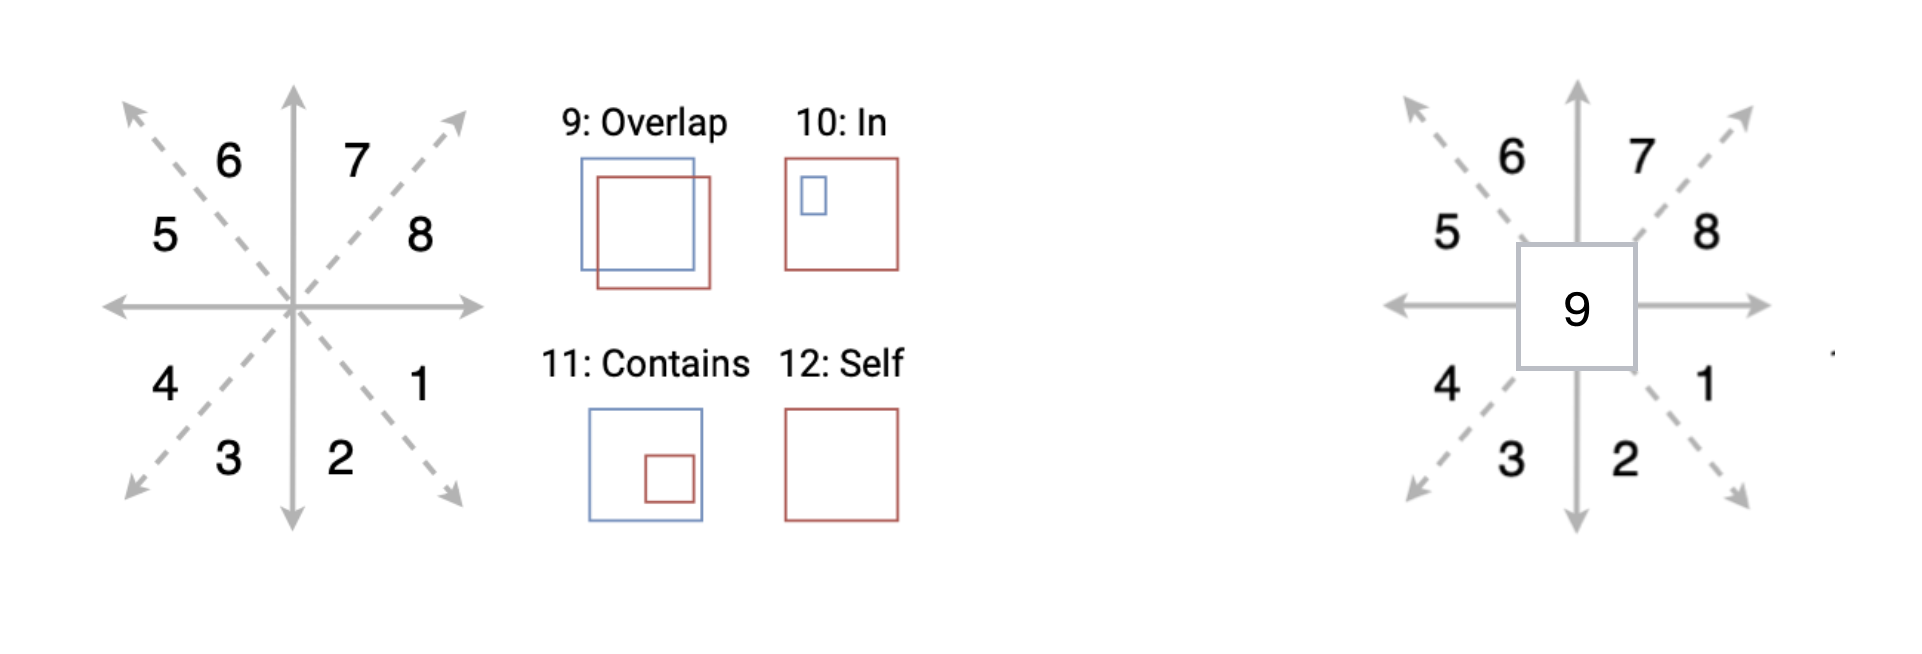
\includegraphics[width=\linewidth]{figures/localization-aware.png}
  \caption{Positional Relationships. (left) Space of potential positional relationship between object/OCR and object/OCR. (right) Space of potential positional relationship between object/OCR and whole image.}
  \label{fig:localization}
\end{figure}
%%%%%%%%%%%%%%%%%%%%%%%%%%%%%%%%%%%%%%%%%%%%%%%%%%%%
Visual relations are proven to be essential part in either uni-modal visual tasks or multi-modal tasks. Many prior works use GAT to learn the spatial relations between objects in the images. However, such relation-aware GAT is not learned across different modalities. Though model is able to learn the spatial relationship well in visual modality, it is hard to respond to the question correctly. Inspired by the idea of implicit relation, several researchers utilizes the vanilla attention mechanism to explore the potential implicit relationship between object, OCR, and questions, but the cross-modality learning happen after the uni-modal embedding, which may compromise the cross-modality learning of relationships.

We propose a data augmentation method called Localization-aware QA Enrichment. Following SA-M4C\cite{kant2020spatially}, we defines $12$ positional relations which can happen between \texttt{<object, object>}, \texttt{<object, OCR>}, and \texttt{<OCR, OCR>}, shown as Fig.\ref{fig:localization}(left). Since we introduce whole image as a new modality, we also define $9$ positional relations between \texttt{<object, IMG>} or \texttt{<OCR, iMG>}, shown as Fig.\ref{fig:localization}(right). We design two templates of questions respectively:
\begin{enumerate}
    \item Template-1: Is A [relative position] to B?
    \item Template-2: Is C [relative position] to the whole image?
\end{enumerate}

By adding these two types of localization-aware question-answer data, we urge the model to learn positional relationship between different modalities under the natural language supervision.

\subsection{Evaluation Metrics}
Accuracy: the accuracy score between predicted answers and ground truth labels.

Average Normalized Levenshtein Similarity (ANLS): the accuracy metric awards a zero score even when the prediction is only a little different from the target answer. Since no OCR is perfect, \citet{mathew2021docvqa} proposed the metric called ANLS for DocVQA task. Motivated by their work, we would also like to include this metric in our evaluation.

Robustness on Augmented Data (RAD): the proportion of correctly predicted augmented questions among all correctly predicted questions. As demonstrated by \citet{RAD}, RAD is a powerful indicator of model robustness on OOD data. Therefore, we would like to include this as a metric of generalization capabilities.  


\section{Team member contributions}
\paragraph{Hao Wu} contributed to relevant techniques (data augmentation & generalizability), model structure diagrams, encoders, image augmentation, and evaluation metrics.

\paragraph{Jiayi Shen} contributed to related datasets, unimodal baseline analysis, relevant techniques (pretraining, multireference), and encoders.

\paragraph{Yanlin Feng} contributed to unimodal baseline analysis, relevant techniques (answer generation), model fine-tuning, and loss function.

\paragraph{Yinghuan Zhang} contributed to relevant techniques (multitasks, attention mechanisms), model structure description, encoders, decoders, and QA enrichment.

\paragraph{Yuwei Wu} contributed to relevant techniques (multitasks, pretraining), encoders, and model pretraining.

% Please use 
\clearpage
\bibliographystyle{acl_natbib}
\bibliography{references}

%\appendix



\end{document}
